\documentclass[11pt]{article}
\usepackage{graphicx}
\usepackage{amssymb}
\newcommand{\cnum}{CM146}
\newcommand{\ced}{Fall 2017}
\newcommand{\ctitle}[3]{\title{\vspace{-0.5in}\cnum, \ced\\Problem Set #1: #2\\Due #3}}
\usepackage{enumitem}
\newcommand{\solution}[1]{{{\color{blue}{\bf Solution:} {#1}}}}
\usepackage[usenames,dvipsnames,svgnames,table,hyperref]{xcolor}
\usepackage{amsmath}

\renewcommand*{\theenumi}{\alph{enumi}}
\renewcommand*\labelenumi{(\theenumi)}
\renewcommand*{\theenumii}{\roman{enumii}}
\renewcommand*\labelenumii{\theenumii.}


\begin{document}
\ctitle{0}{Math prerequisites}{Jan 18, 2018}
\author{}
\date{}
\maketitle
\vspace{-0.75in}

\section{Problem 1}
Solution:
\begin{equation*}
\frac{\partial y}{\partial x}
= \sin(z) \frac{\partial}{\partial x} xe^{-x}
= \sin(z) (1 - x) e^{-x}.
\end{equation*}

\newpage
\section{Problem 2}
\begin{enumerate}
\item
Solution:
\begin{equation*}
  y^Tz = \begin{pmatrix}
    1 &3 \end{pmatrix} \begin{pmatrix} 2 \\ 3 \end{pmatrix} = \begin{pmatrix} 11 \end{pmatrix}.
\end{equation*}
\item
Solution:
\begin{equation*}
  Xy = \begin{pmatrix}
    2 &4\\
    1 &3 \end{pmatrix} \begin{pmatrix} 1 \\ 3 \end{pmatrix}
  = \begin{pmatrix} 14 \\ 10 \end{pmatrix}.
\end{equation*}
\item
Solution:
\begin{equation*}
  X^{-1} = \frac{1}{2} \begin{pmatrix} 3 &-4\\ -1 &3 \end{pmatrix}\\
  = \begin{pmatrix} 3/2 &-2\\ -1/2 &3/2 \end{pmatrix}.
\end{equation*}
\item
Solution:
\begin{equation*}
rank(X) = 2.    
\end{equation*}
\end{enumerate}
\newpage
\section{Problem 3}
\begin{enumerate}
\item
  Solution:
  \begin{equation*}
    \frac{1 + 1 + 0 + 1 + 0}{5} = 3/5.
  \end{equation*}
\item
  Solution:
  \begin{equation*}
    \frac{(1-3/5)^2 + (1-3/5)^2 + (0-3/5)^2 + (1-3/5)^2 + (0-3/5)^2}{5-1}
    = \frac{4 + 4 + 9 + 4 + 9}{4*25} = 0.3.
  \end{equation*}  
\item
  Solution:
  \begin{equation*}
    \frac{1}{2^5}.
  \end{equation*}
\item
  Solution:
  \begin{align*}
    P &= p^3(1-p)^2.\\
    0 &= \frac{dP}{dp} = 3p^2(1-p)^2 - 2p^3(1-p) \Rightarrow p \in \{0, 1, 3/5\}.
  \end{align*}
  Maximum for $p = 3/5$.

\item
  Solution:
  \begin{equation*}
    \frac{0.1}{0.1 + 0.15} = \frac{2}{5}.
  \end{equation*}
\end{enumerate}
\newpage
\section{Problem 4}
\begin{enumerate}
\item
  False
\item
  True
\item
  False
\item
  False
\item
  True
\end{enumerate}
\newpage
\section{Problem 5}
\begin{enumerate}
\item (v)
\item (iv)
\item (ii)
\item (i)
\item (iii)
\end{enumerate}
\newpage
\section{Problem 6}
\begin{enumerate}
\item
  Mean: $p$
  
  Variance: $p(1-p)$
\item
  $Var(X+2) = \sigma^2$

  $Var(2X) = 4Var(X) = 4\sigma^2$
\end{enumerate}
\newpage
\section{Problem 7}
\begin{enumerate}
\item
  Both.
  \[\lim_{x \rightarrow \infty} \frac{lg(x)}{ln(x)} = \lim_{x \rightarrow \infty} 1/ln(2) < \infty.\]
  \[\lim_{x \rightarrow \infty} \frac{ln(x)}{lg(x)} = \lim_{x \rightarrow \infty} 1/lg(e) < \infty.\]
\item
  $g(n) = O(f(n))$ only.
  \[\lim_{x \rightarrow \infty} \frac{g(x)}{f(x)} = \lim_{x \rightarrow \infty} \frac{x^{10}}{3^x} = 0 < \infty.\]
  \[\lim_{x \rightarrow \infty} \frac{f(x)}{g(x)} = \lim_{x \rightarrow \infty} \frac{3^x}{x^{10}} = \infty.\]
\item
  $g(n) = O(f(n))$ only.
  \[\lim_{x \rightarrow \infty} \frac{g(x)}{f(x)} = \lim_{x \rightarrow \infty} \left(\frac{2}{3}\right)^n = 0 < \infty.\]
  \[\lim_{x \rightarrow \infty} \frac{f(x)}{g(x)} = \lim_{x \rightarrow \infty} \left(\frac{3}{2}\right)^n = \infty.\]

\item Algorithm:
  \begin{enumerate}
  \item Set \texttt{low} to $0$ and \texttt{high} to $n$.
  \item Set \texttt{mid} to $\frac{\texttt{low} + \texttt{high}}{2}$.
  \item If \texttt{array[floor(mid)]} is $1$ then set \texttt{high} to
    \texttt{floor(mid)},
    else set \texttt{low} to \texttt{floor(mid)}.
  \item If \texttt{high-low == 1} then transition happens between
    \texttt{high} and \texttt{low}, else go to (ii).
  \end{enumerate}
  Explanation: \texttt{array[low]} always remains $0$ and \texttt{array[high]}
  always remains $1$. So, once $\texttt{high} - \texttt{low} == 1$ we know the
  transition happens in between the two. $\texttt{high} - \texttt{low}$ will
  converge to $1$, because $\texttt{floor(mid)} < \texttt{high}$ and
  $\texttt{floor(mid)} > \texttt{low}$ whenever
  $\texttt{high} - \texttt{low} > 1$, so the difference becomes smaller on
  every step.
\end{enumerate}
\newpage
\section{Problem 8}
\begin{enumerate}
\item
Proof for general case:
\begin{align*}
  \mathbb{E}[XY] &= \int_a^b\int_c^d xyp_{XY}(xy)\,dy \,dx\\
  &= \int_a^b\int_c^d xyp_{X}(x)p_Y(y)\,dy \,dx\\
  &= \int_a^b xp_{X}(x) \,dx \int_c^d yp_{Y}(y) \,dy\\
  &= \mathbb{E}[X] \mathbb{E}[Y].
\end{align*}
\item
  
  Let $X_i$ be $1$ if the result of the $i^{th}$ roll is $3$ and $0$ otherwise.
  Therefore the $X_i$'s are independent Bernoulli random variables with
  $p=1/6$, \textit{i.e.} they are independent identically distributed random
  variables.
  
  Below I used the CLT because I though it was more precise, but relized it has
  the same flaws as LLN. By Strong LLN $\sum X_i \rightarrow N/6$ almost surely
  as $N \rightarrow \infty$. Therefore, we expect $1000$ $3$'s.

  Therefore, by the Central Limit Theorem, in the limit of large $N$
  \[\frac{1}{\sqrt{6000}} \sum_{i=1}^{6000} (X_i - 1/6) \sim \mathcal{N}(0, 5/36)\]
  \textit{i.e.,}
  \[\frac{1}{6000}\sum_{i=1}^{6000} X_i \sim \mathcal{N}\left(\frac{1}{6}, \frac{5}{36\cdot 6000}\right)\]
  \[\sum_{i=1}^{6000} X_i \sim \mathcal{N}\left(1000, \frac{5 \cdot 6000}{36}\right)\]  
So, $\sigma \approx 28.86$. Therefore, there is a $95\%$ probability that there
will be between $942$ and $1058$ $3$'s.
\item
  Direct consequence of Central Limit Theorem, which states that in the limit
  of large $n$:
  \[\sqrt{n} \left(\frac{1}{n}\sum_{i=1}^{6000} X_i - \mu\right) \sim \mathcal{N}(0, \sigma^2)\]
  where $Var(X_i) = \sigma^2$ and $\mathbb{E}(X_i) = \mu$.
\end{enumerate}
\newpage
\section{Problem 9}
\begin{enumerate}
\item
  \begin{enumerate}
  \item Circle centered at the origin with radius $1$.
  \item The $x$- and $y$-axis.
  \item Square with diagonals aligned with the $x$- and
    $y$-axis and side length equal to $\sqrt{2}$.
  \item Square centered at origin, with sides parallel to the $x$- and $y$-axis
    and side length equal to $1$.
  \end{enumerate}
\item
  \begin{enumerate}
    \item
      $\lambda$ is called an eigenvalue of a square matrix $A$ if and only if
      there exists a non-zero vector $\vec{v}$ such
      that $A\vec{v} = \lambda \vec{v}$.
      All such $\vec{v}$ are called eigenvectors of $A$ associated with
      $\lambda$.
    \item The eigenvalue $\lambda = 3$ has eigenvector of the form
      $k\begin{pmatrix} 1 \\ 1\end{pmatrix}$ for any $k \in \mathbb{R}\backslash \{0\}$.
    \item
      For any $\lambda$ eigenvalue of $A$ and associated eigenvector $\vec{v}$
      \begin{align*}
        &A\vec{v} = \lambda \vec{v}\\
        \Rightarrow &(A - \lambda I) \vec{v} = \vec{0}\\
        \Rightarrow &(A^{k-1}I^0 + ... + A^0I^{k-1})(A - \lambda I) \vec{v} = \vec{0}\\
        \Rightarrow &(A^k - (\lambda I)^k) \vec{v} = \vec{0}\\
        \Rightarrow &A^k\vec{v} = \lambda^k \vec{v}.
      \end{align*}
      Due to commutativity of identity matrix.
  \end{enumerate}
\item
  \begin{enumerate}
  \item First,
    \[a^Tx = \begin{pmatrix} a_1 &a_2 &\dots &a_n\end{pmatrix}
      \begin{pmatrix}
        x_1\\
        x_2\\
        \vdots\\
        x_n
      \end{pmatrix} = a_1x_1 + ... + a_nx_n.\]
      So,
      \begin{align*}
        \frac{\partial a^Tx}{\partial x} &=
        \begin{pmatrix}
          \frac{\partial}{\partial x_1} &... &\frac{\partial}{\partial x_2}
        \end{pmatrix} (a_1x_1 + ... + a_nx_n)\\
        &= \begin{pmatrix} a_1 &a_2 &\dots &a_n \end{pmatrix}
      \end{align*}
    \item
      \begin{equation*}
        \begin{pmatrix}
          x_1 &x_2 &\dots &x_n         
        \end{pmatrix}
        \begin{pmatrix}
          A_{11} &\dots &A_{1n}\\
          \vdots &\ddots &\vdots\\
          A_{n1} &\dots &A_{nn}          
        \end{pmatrix}
        \begin{pmatrix}
          x_1 \\
          x_2 \\
          \vdots \\
          x_n         
        \end{pmatrix} =
        \sum_{i, j} A_{ij} x_i x_j.
      \end{equation*}
      \begin{equation*}
        \frac{\partial x^T A x}{\partial x} =
        \begin{pmatrix}
          A_{11}x_1 + \sum_{j \neq 1}(A_{j1} + A_{1j}) x_j
          &\dots
          &A_{nn}x_n + \sum_{j \neq n}\sum_j (A_{jn} + A_{nj}) x_j
        \end{pmatrix}
      \end{equation*}
      \begin{equation*}
        \frac{\partial^2 x^T A x}{\partial x^2} =
        \begin{pmatrix}
          A_{11} &\dots &A_{1n}\\
          \vdots &\ddots &\vdots\\
          A_{n1} &\dots &A_{nn}          
        \end{pmatrix} = A.
      \end{equation*}
  \end{enumerate}
\item
  \begin{enumerate}
  \item
    \begin{align*}
      \omega^T(x_1 - x_2) &= \omega^Tx_1 - \omega^Tx_2\\
      &= (\omega^Tx_1 + b) - (\omega^Tx_2 + b) = 0.
    \end{align*}
  \item
    The distance will be equal to the magnitude of the vector $\vec{v}$ which is
    orthogonal to the
    line, such that the vector itself belongs to the line, \textit{i.e.}
    \begin{equation*}
      \vec{v} = k\omega, \quad \omega^T\vec{v} + b = 0.
    \end{equation*}
    For $k = -b^{-1}$ both equations are satisfied (uniquely since two lines
    intersect in at most one point) and the required magnitude is obtained.
  \end{enumerate}
\end{enumerate}
\newpage
\section{Problem 10}
\begin{enumerate}
\item
  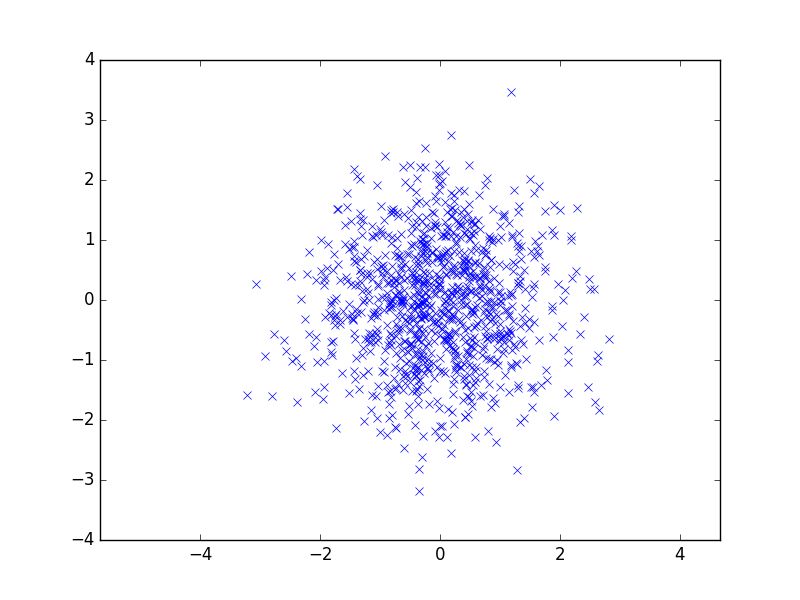
\includegraphics[height=5cm]{fig1.png}
\item
  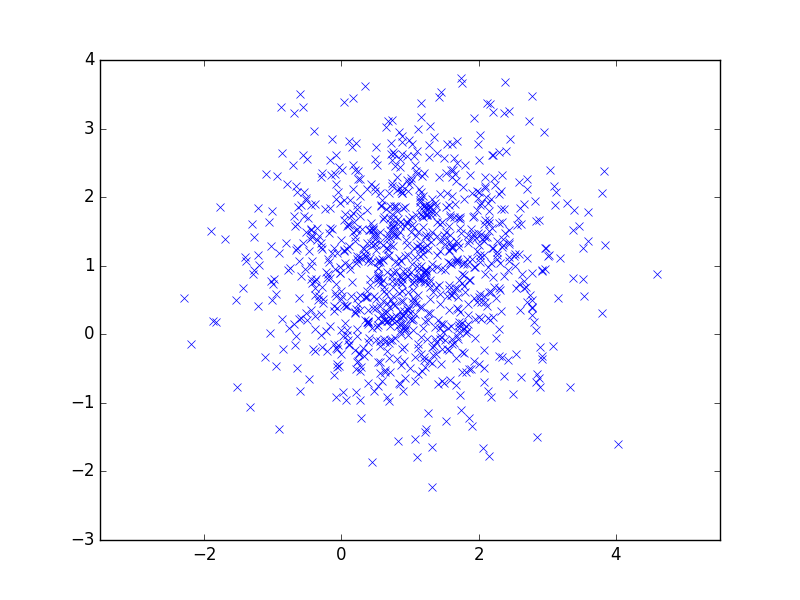
\includegraphics[height=5cm]{fig2.png}
\item
  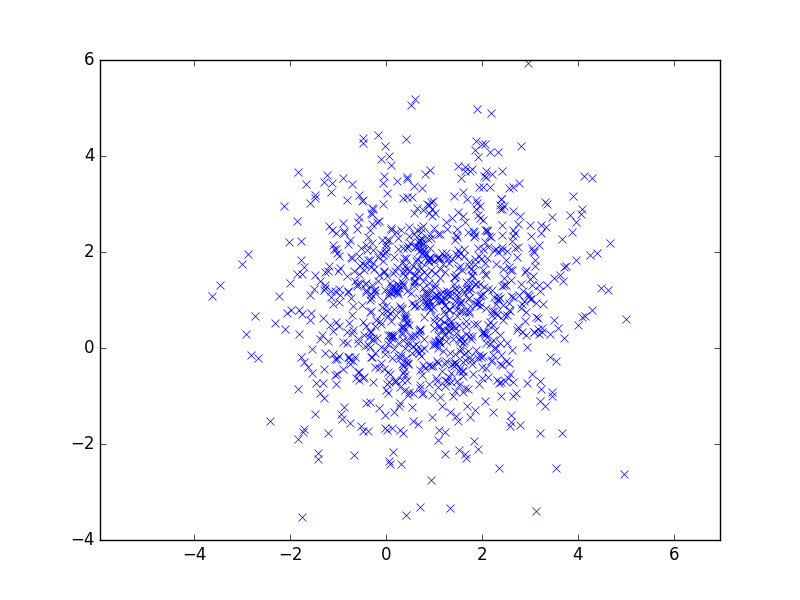
\includegraphics[height=5cm]{fig3.png}
\item
  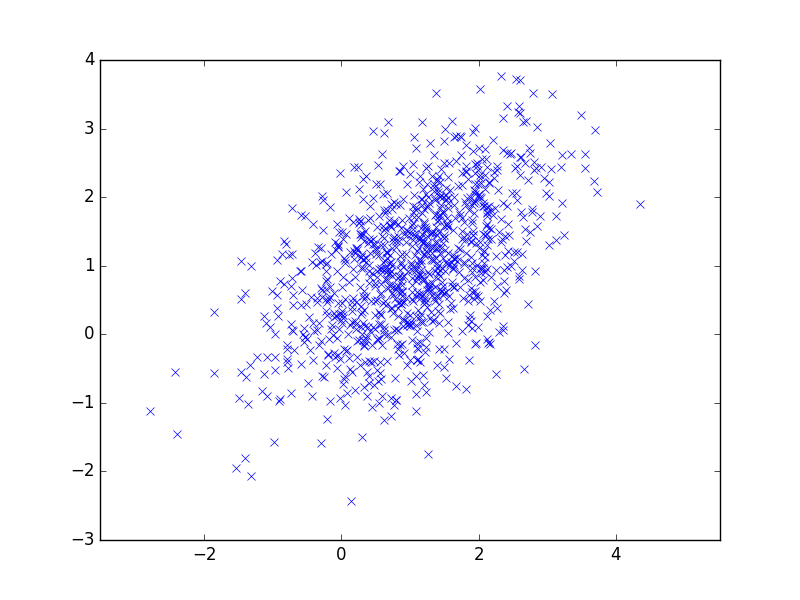
\includegraphics[height=5cm]{fig4.png}
\item
  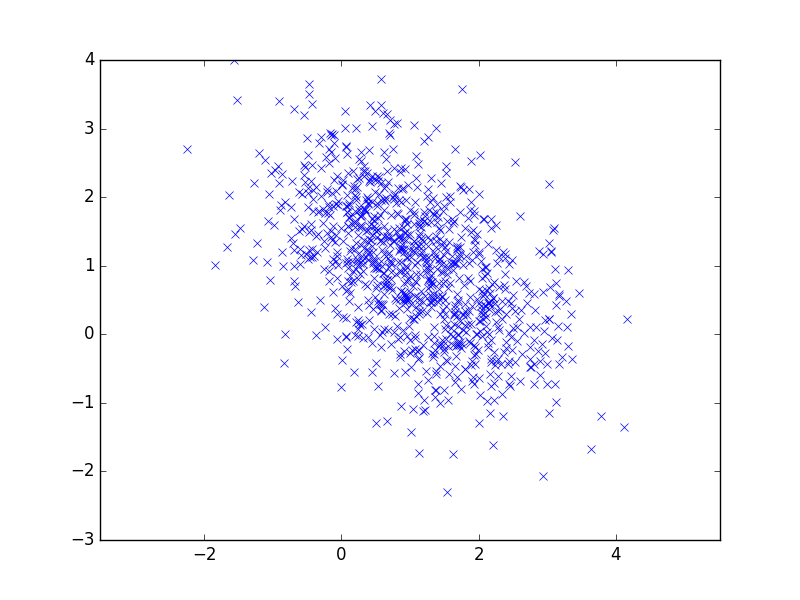
\includegraphics[height=5cm]{fig5.png}
\end{enumrate}
\newpage
\section{Problem 11}
\begin{equation*}
  \begin{pmatrix}
    0\\
    1
  \end{pmatrix}
\end{equation*}
\newpage
\section{Problem 12}
\begin{enumerate}
\item The MNIST Database
\item http://yann.lecun.com/exdb/mnist/
\item The dataset contains images of handwritten digits. The content of the
  image defines the features for the specific datapoint, while each datapoint
  also has a label associated with it that specifies which digit is written in
  the image.
\item One training set contains 60,000 and the other 10,000 datapoints.
\item There is one feature for each example: the image.
\end{enumerate}
\end{document}
